% LTeX: language=sl-SI
\section{Učinkovitost Schnorrovega, večstranskega Schnorrovega in MuSig2 podpisa}
\label{sec:primerjava}
Naravno vprašanje, ki se pojavi ob omembi večstranskega Schnorrovega podpisa podskupine z odgovornostjo
ali pa MuSig2, je, kakšne prednosti ponujata pred uporabo več navadnih Schnorrovih podpisov. Najočitnejša
prednost je, da večstranski podpis vrne en sam podpis, ki je primerljivo dolg s Schnorrovim, medtem
ko uporaba individualnih podpisov pomeni, da mora preverjevalec preveriti toliko podpisov, kot je
velika skupina. Ta prednost večstranskega podpisa je posebej pomembna v primerih, ko je preverjevalčev
čas zelo omejen ali drag. Odličen primer je pri vseh aplikacijah, ki temeljijo na tehnologiji veriženja
blokov, kjer preverjanje podpisov poteka ">na verigi"<, torej je za vsako operacijo potrebno plačati.

Seveda pa je potrebno omeniti tudi slabosti večstranskih podpisov v primerjavi z navadnimi. Najbolj
očitna je, da morajo podpisniki med seboj komunicirati, kar lahko pomeni velike izgube časa. Uporabna
vrednost večstranskih podpisov torej sloni na primerih, kjer je komunikacija enostavna, čas in
računska moč preverjevalca pa izjemno dragocena (ponovno so odličen primer aplikacije, ki temeljijo
na veriženju blokov).

\subsection{Empirična analiza}
Za empirično potrditev zgornjih trditev smo razvili program, ki implementira vse podpise v nekoliko
poenostavljenem okolju. Zanemarili smo čas komunikacije pri vseh verzijah podpisov, saj je to nezanesljiv
podatek, ki je odvisen od okolja. Cilj primerjave je videti, kako se razlikuje čas izvedbe posameznih
komponent podpisov pri različnem številu podpisnikov.

Zaradi zanemarjanja komunikacije pričakujemo, da bodo časi podpisovanja in generiranja ključev pri
večstranskih podpisih nekoliko krajši, kot so v resnici, čas preverjanja pa bo odražal realno stanje.

Podpise smo implementirali v programskem jeziku Go, vsa izvorna koda je na voljo na
\url{https://github.com/timkalan/magisterij}. Poskusi so bili izvedeni na računalniku z Apple M1 Pro
procesorjem in 16 GB RAM-a. Vsak poskus smo ponovili šestkrat, da smo dobili stabilne rezultate, ki
smo jih nato povprečili. Za dodatno nazornost smo izračunali še standardne odklone vseh poskusov.
Vsi grafi prikazujejo povprečne vrednosti skupaj s standardnim odklonom.

Poskusi so bili narejeni z $1, 2, 5, 10, 20, 30, \dots, 200$ podpisniki. Velikost parametra $q$, ki
določa grupo, iz katere je generator, je bila $256$ bitov. Za grupo smo izbrali multiplikativno grupo
naravnih števil modulo $p$, kjer je $p-1$ večkratnik parametra $q$. Za zgoščevalno funkcijo smo
uporabili \texttt{SHA-256}, ki je bila izbrana zaradi velike razširjenosti.

\subsubsection{Generiranje ključev}
Generiranje ključev se pri vseh podpisih začne enako. Vsi podpisniki morajo izbrati naključne zasebne
ključe in generirati javne ključe kot $X_i = g^{s_i} \pmod p$. Tu se generiranje ključev za navaden
Schnorrov podpis in MuSig2 konča, pri večstranskem podpisu pa je potrebno še ustvariti dokaze znanja brez
razkritja znanja, jih poslati vsem ostalim podpisnikom in preveriti njihovo veljavnost. To je seveda
zelo veliko dodatnega dela, ki pa ga je za določeno skupino potrebno opraviti samo enkrat (kot je
tudi potrebno samo enkrat generirati par ključev pri navadnem Schnorrovem podpisu).

\begin{figure}[ht]
  \centering
  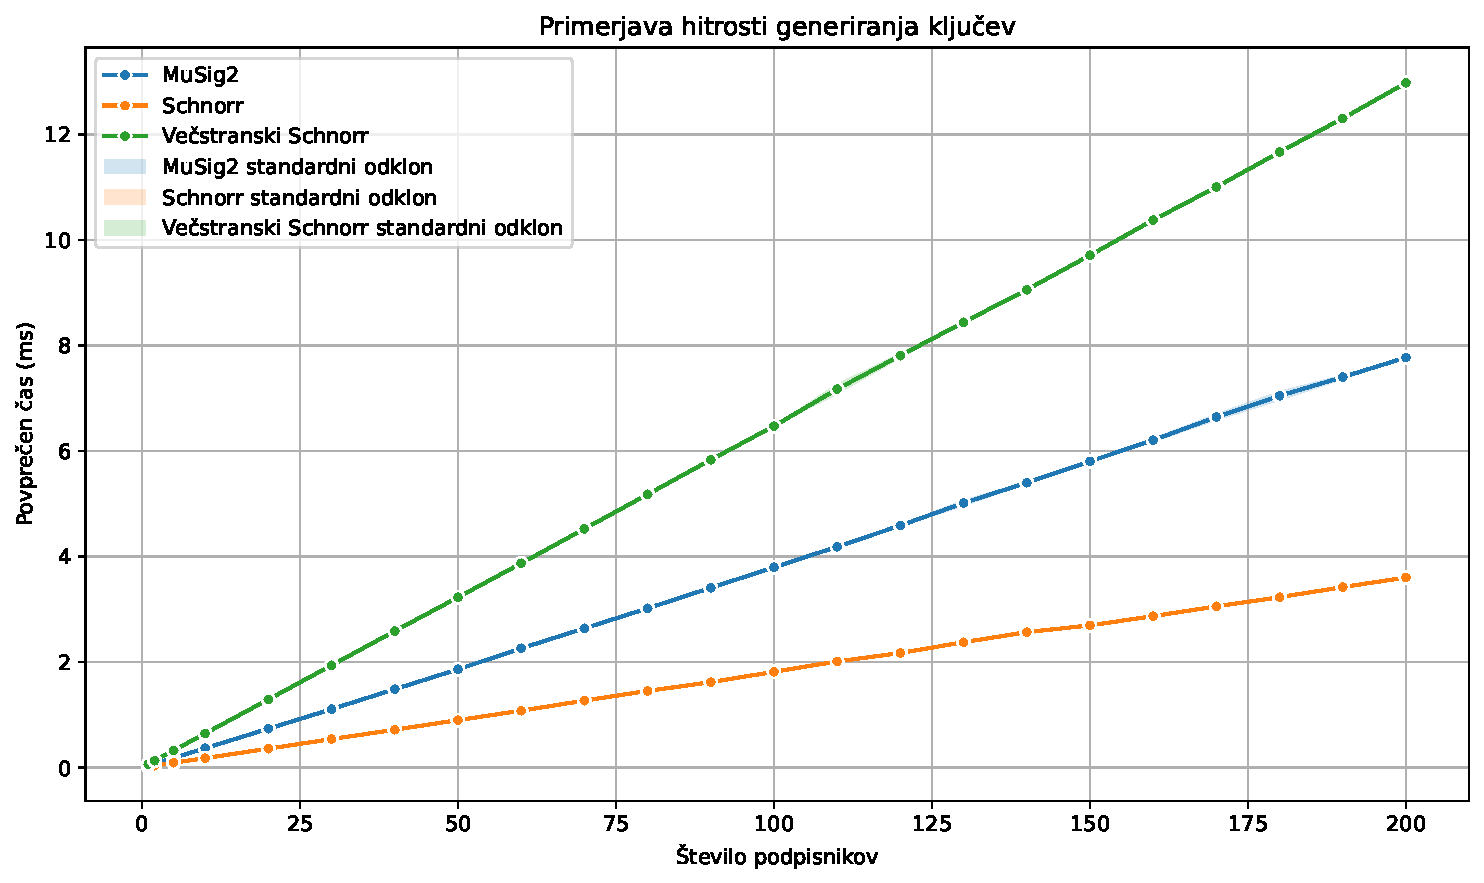
\includegraphics[width=0.8\textwidth]{images/benchmark_KeyGeneration.pdf}
  \caption[Generiranje ključev.]{Primerjava časov generiranja ključev pri Schnorrovem, večstranskem
    Schnorrovem in MuSig2 podpisu. Prikazan je skupen čas generiranja ključev za vse podpisnike.}
  \label{fig:generiranje}
\end{figure}

Kot je razvidno iz slike~\ref{fig:generiranje}, je čas generiranja ključev pri večstranskem Schnorrovem
podpisu mnogo daljši, ne glede na količino podpisnikov. MuSig2 porabi enako časa kot Schnorrov podpis,
vendar smo vključili še čas agregacije ključev, zato je potreben še dodaten čas. Rast
zahtevnosti v vseh primerih je linearna s številom podpisnikov, a je vseeno hitrejša pri večstranskih
podpisih. V praksi je za večstranski Schnorrov podpis potrebno še več časa, saj smo tu zanemarili čas
komunikacije, ki je v tem primeru linearen s številom podpisnikov. Ker pa se mora ta komunikacija
zgoditi samo enkrat, jo tu zanemarimo (ključe skupina ustvari le ob začetku sodelovanja). Za ponazoritev
razlike: pri $100$ podpisnikih se za generiranja ključev pri navadnem podpisu porabita približno $2$
milisekundi, pri MuSig2 $4$ milisekunde, pri večstranskem Schnorrovem pa $6$ milisekund.

Generiranje ključev predstavlja veliko prednost navadnega Schnorrovega podpisa, vendar
si moramo zapomniti, da je to postopek, ki ga mora skupina opraviti le enkrat, hkrati pa ne obremenjuje
preverjevalca. Če smo torej v situaciji, kjer mora ista skupina podpisnikov velikokrat skupaj podpisati
sporočila, je čas generiranje ključev zanemarljiv, v primeru enkratnih skupin pa je morda smiselno
razmišljati o uporabi navadnega Schnorrovega podpisa.

\subsubsection{Podpisovanje}
Pri podpisovanju največjo razliko med podpisi naredi potreba po komunikaciji med podpisniki pri
večstranskih podpisih. Zahtevno je predvsem to, da so za ustvarjanje enega podpisa potrebni trije
krogi komunikacije za večstranski Schnorrov podpis:
\begin{itemize}
    \item izmenjava zavez $X_i$,
    \item izmenjava skupne zaveze $\tilde{X}$
    \item in izmenjava izziva $e$,
\end{itemize}
in dva kroga pri MuSig2:
\begin{itemize}
    \item izmenjava zavez $X_{1, i, j}$,
    \item izmenjava delnih podpisov $y_i$.
\end{itemize}
Če pa komunikacijo zanemarimo, pa je čas podpisovanja enak za Schnorrov in večstranski Schnorrov podpis,
kot je razvidno tudi iz naše analize na sliki~\ref{fig:podpisovanje} (kjer smo zanemarili čas
komunikacije). Vsa računska kompleksnost pri MuSig2 pa se pojavi ravno v času podpisovanja, zato v
povprečju porabi dvakrat več časa kot ostali dve shemi. Rezultati tega preizkusa na prvi pogled
nakazujejo na pomanjkljivost MuSig2 v primerjavi z večstranskim Schnorrovim podpisom, vendar je ta
prednost varljiva, saj se glavnina časa pri ustvarjanju večstranskih podpisov porabi za komunikacijo.
V primeru, da bi upoštevali čas komunikacije, bi dobili bolj realen rezultat, torej veliko prednost
MuSig2, ki potrebuje le dva kroga komunikacije.

\begin{figure}[ht]
  \centering
  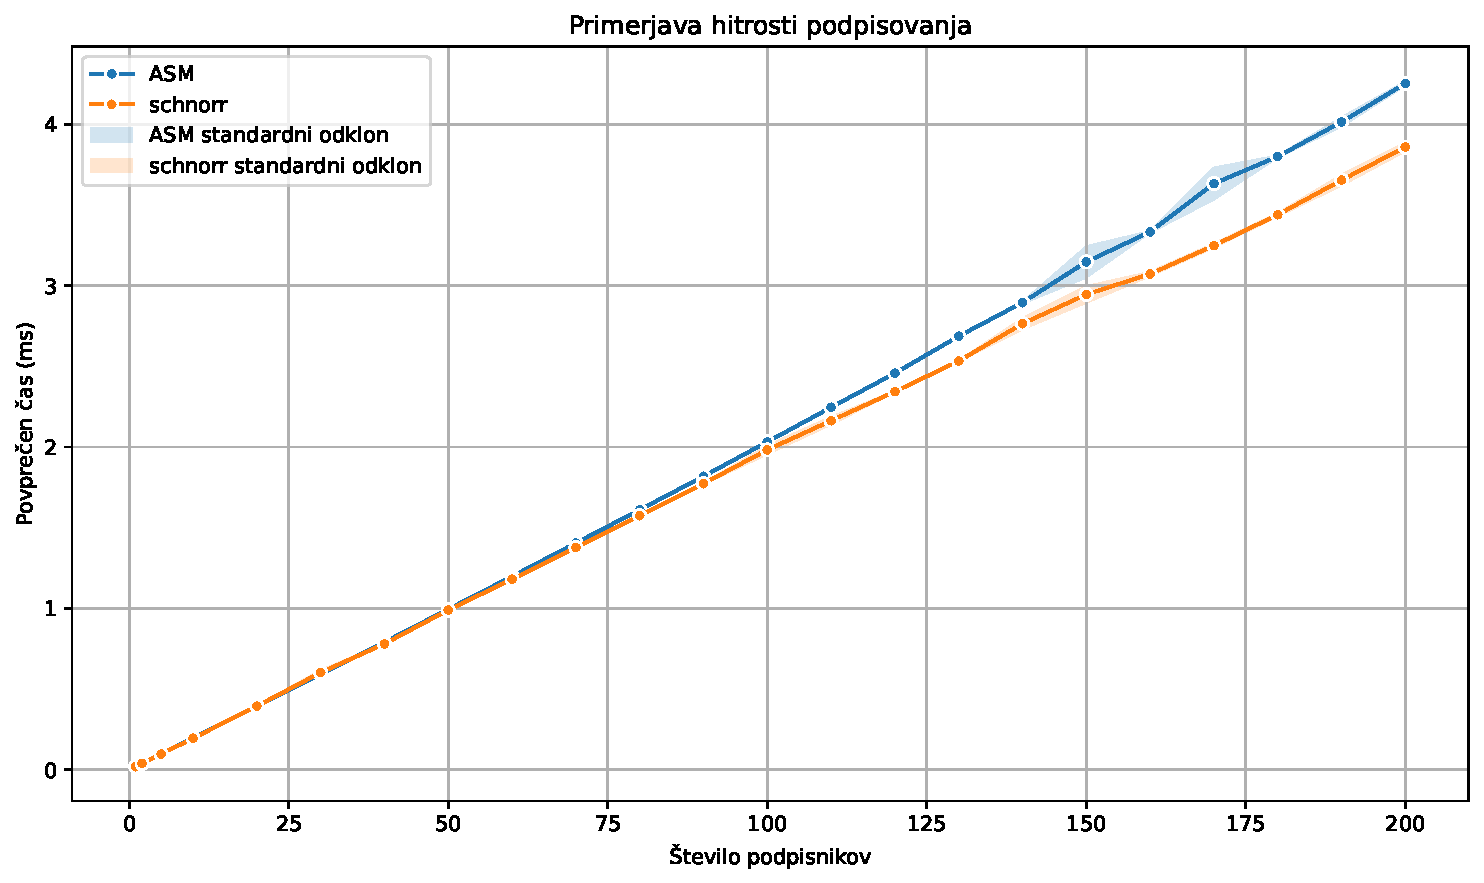
\includegraphics[width=0.8\textwidth]{images/benchmark_Signing.pdf}
  \caption[Podpisovanje.]{Primerjava časov podpisovanja pri Schnorrovem, večstranskem Schnorrovem
      in MuSig2 podpisu. Prikazan je skupen čas podpisovanja za vse podpisnike.}
  \label{fig:podpisovanje}
\end{figure}

Graf torej odraža čas, ki ga porabi računalnik za računanje, zanemari pa čas komunikacije. Teoretično
je čas za komunikacijo konstanten, če lahko podpisniki hkrati pošljajo in prejemajo več sporočil.
V praksi pa čas zavisi od mnogih pogojev, kot so hitrost povezave, število podpisnikov in stabilnost
povezave.

\subsubsection{Preverjanje}
Ena največjih prednosti večstranskih podpisov je, da podpis vedno ostane enako dolg kot navaden podpis
– ne glede na število podpisnikov. Prednost je sploh očitna pri MuSig2, saj mora preverjevalec preveriti
samo en navaden Schnorrov podpis. Pri večstranskem Schnorrovem podpisu ima še dodano nalogo preverjanja
ustreznosti Merklovih korenov, kar pa je relativno hitro in učinkovito.

Navaden Schnorrov podpis zahteva preverjanje vsakega podpisa posebej, kar pomeni, da efektivno
dolžina podpisa raste linearno s številom podpisnikov. To pomeni, da tako raste tudi čas preverjanja.
Prednost večstranskih podpisov lahko vidimo na sliki~\ref{fig:preverjanje}. Zahtevnost preverjanja
navadnega Schnorrovega podpisa narašča mnogo hitreje, kot zahtevnost večstranskega. Kljub veliki
prednosti večstranskega Schnorrovega podpisa, vidimo, da zahtevnost vseeno ni konstantna, temveč tudi
linearno narašča. To je zato, ker trenutna implementacija podpisa vsakič, ko se podpis preveri, ponovno
konstruira Merklovo drevo. V praksi to za zaporedne podpise enakih skupin ne bi bilo potrebno,
saj bi preverjevalec enostavno lahko shranil Merklovo drevo, kar pomeni, da bi bilo preverjanje še
toliko bolj učinkovito.

Tu se odlično prikaže prednost MuSig2, saj je čas preverjanja konstanten, ne glede na število
podpisnikov. Cena dodatne učinkovitosti pa je dejstvo, da MuSig2 nima lastnosti odgovornosti, ki jo
omogoča Merklovo drevo. Pri uporabi v praksi je tako potrebno presoditi, ali je bolj ključnega pomena
odgovornost ali pa učinkovitost (sploh za preverjevalca).

\begin{figure}[ht]
  \centering
  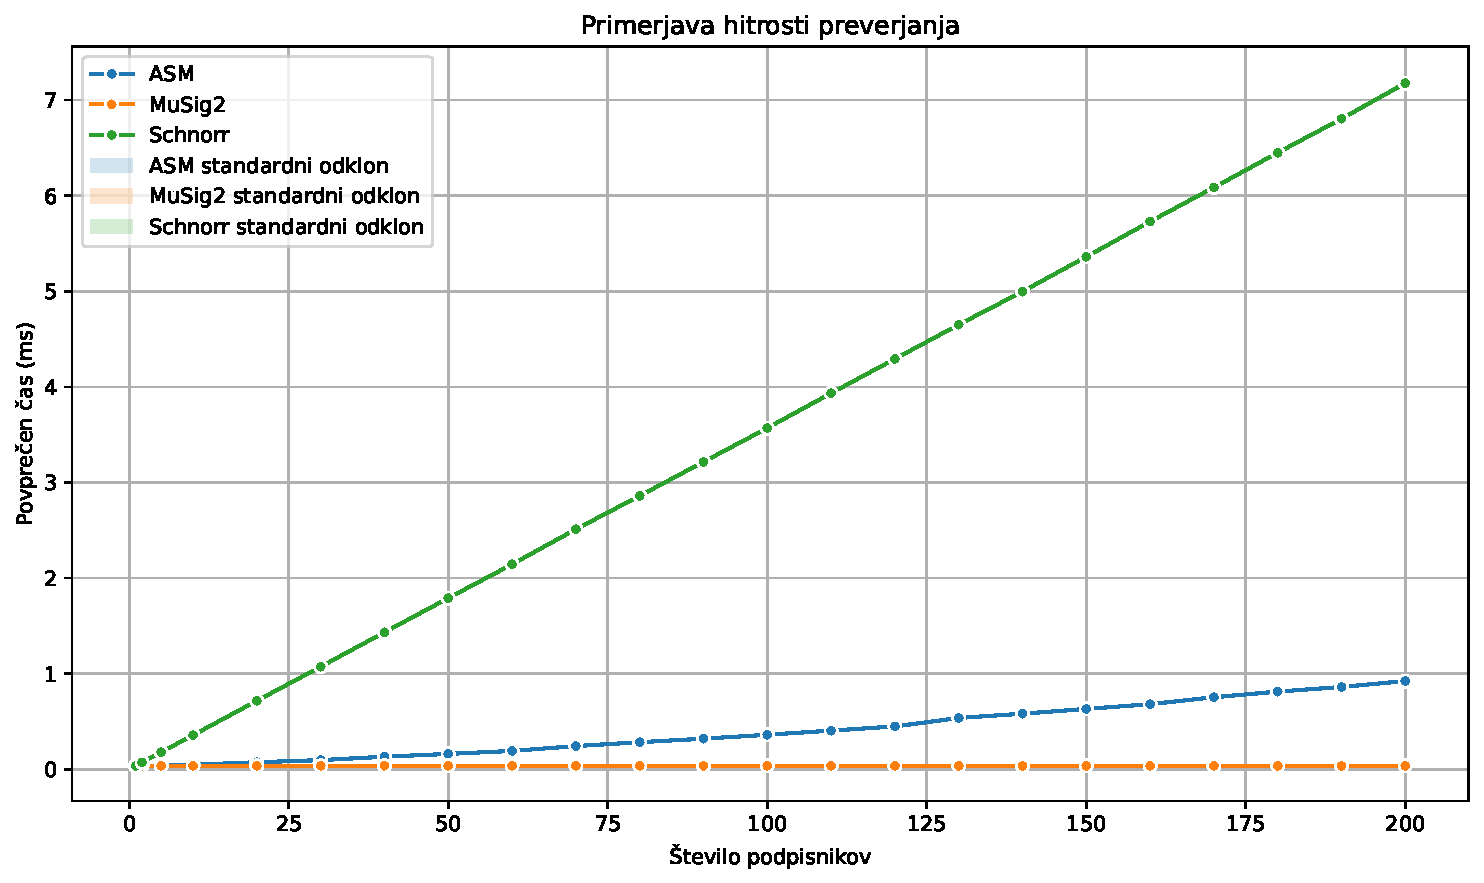
\includegraphics[width=0.8\textwidth]{images/benchmark_Verification.pdf}
  \caption[Preverjanje.]{Primerjava časov preverjanja veljavnosti podpisov pri Schnorrovem, večstranskem
    Schnorrovem in MuSig2 podpisu. Prikazan je skupen čas preverjanja za vse podpisnike.}
  \label{fig:preverjanje}
\end{figure}

\subsubsection{Celotni podpis}
Če združimo vse operacije -- torej generiranje ključev, podpisovanje in preverjanje -- med podpisi
ni bistvenih razlik. Navaden Schnorrov podpis je vseeno najučinkovitejši, ker večstranska podpisa
zahtevata veliko računanja za generiranje ključev oz.\ podpisovanje. To se jasno vidi na
sliki~\ref{fig:celotni}. Seveda pa je to nekoliko nerealistična primerjava, saj nas redko zanima
celoten čas, ki ga bodo porabili različni deležniki različno mnogokrat (npr.\ ključi bodo za neko
skupino generirani le enkrat, porabljen čas podpisnikov in preverjevalca moramo obravnavati drugače).
Kljub temu nam da dobro predstavo o tem, kako se čas podpisovanja različnih podpisov spreminja s
številom podpisnikov in kako na ta čas vplivajo posamezne operacije podpisa.

\begin{figure}[ht]
  \centering
  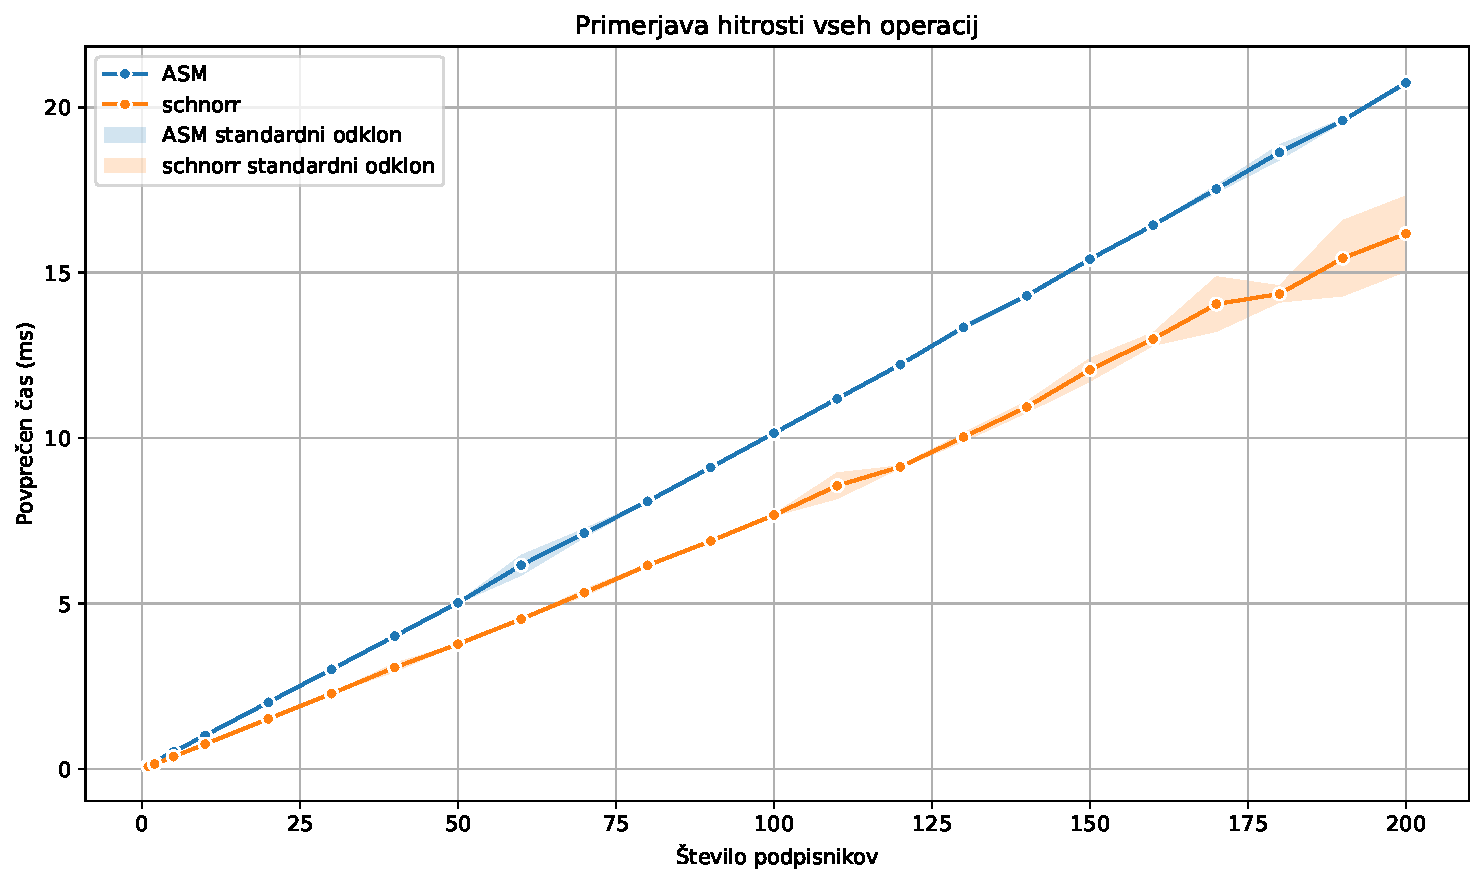
\includegraphics[width=0.8\textwidth]{images/benchmark_All.pdf}
  \caption[Celotni podpis.]{Primerjava časov celotnega postopka izvedbe podpisne sheme pri Schnorrovem,
      večstranskem Schnorrovem in MuSig2 podpisu. Prikazan je skupen čas celotnega postopka za vse
      podpisnike.}
  \label{fig:celotni}
\end{figure}

Za konec lahko analiziramo še situacijo, kjer bi ustaljena skupina podpisnikov sodelovala dlje časa,
torej bi samo enkrat generirali ključe, nato pa se skupno podpisovali poljubno mnogokrat. V tem
primeru zanemarimo čas generiranja ključev, ki se zgodi le na začetku. Slika~\ref{fig:podpis-preverjanje}
jasno prikaže prednost večstranskih podpisov v tem primeru. Za najbolj učinkovitega se zdi večstranski
Schnorrov podpis, vendar je prednost ponovno varljiva. MuSig2 res porabi več časa za računanje, vendar
prihrani eno tretjino komunikacije, kar je v realnem svetu glavni faktor, ki odloča o učinkovitosti.

\begin{figure}[ht]
  \centering
  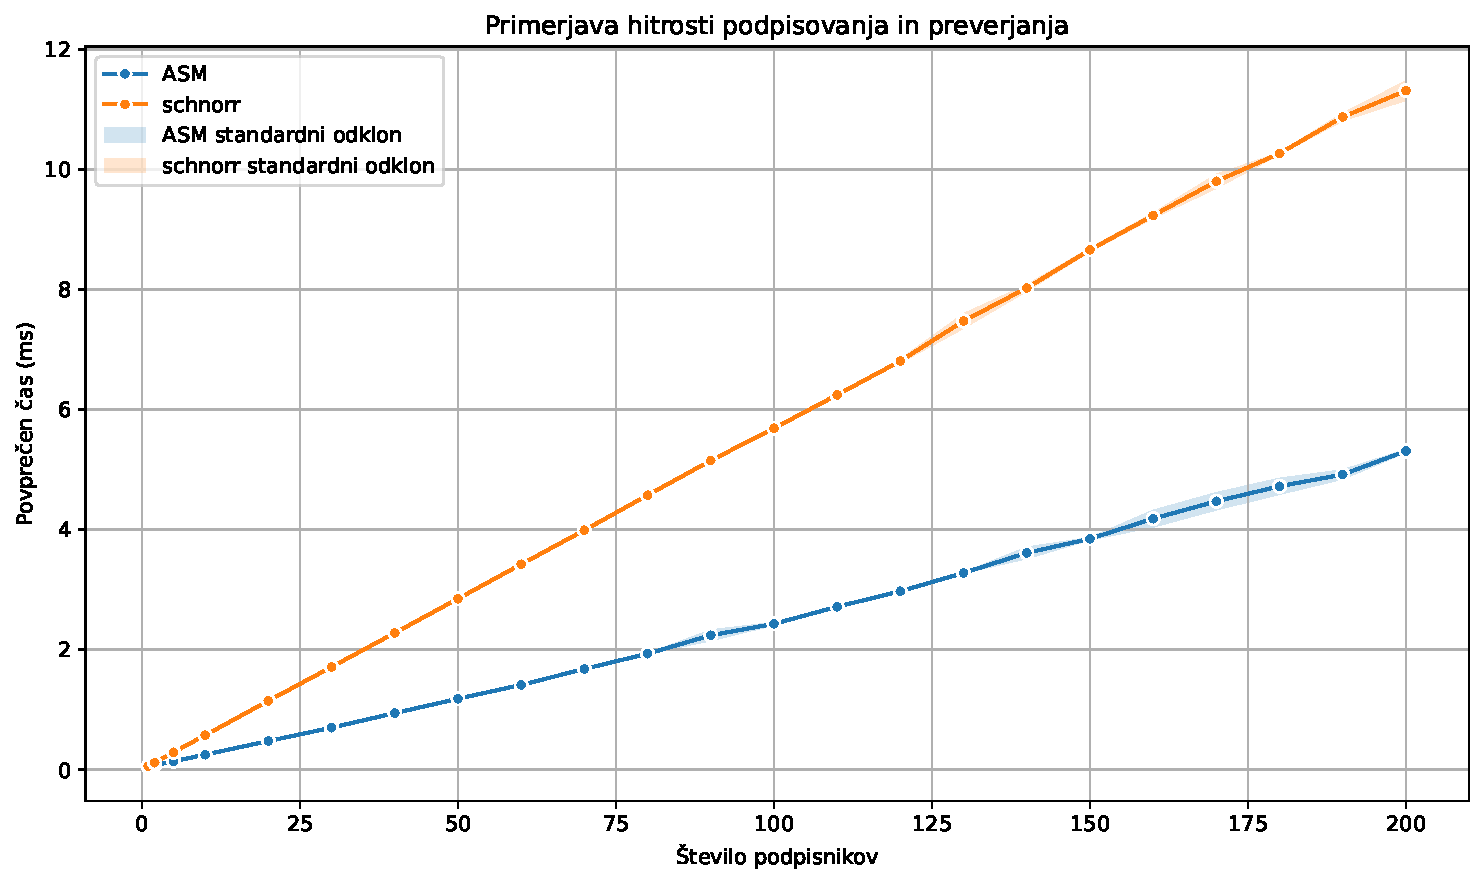
\includegraphics[width=0.8\textwidth]{images/benchmark_SigningVerification.pdf}
  \caption[Podpisovanje in preverjanje.]{Primerjava časov podpisovanja in preverjanja veljavnosti
    podpisov pri Schnorrovem, večstranskem Schnorrovem in MuSig2 podpisu. Prikazan je skupen čas
    podpisovanja in preverjanja za vse podpisnike.}
  \label{fig:podpis-preverjanje}
\end{figure}

\subsection{Razprava}
Na podlagi rezultatov vidimo, da so večstranski podpisi lahko zelo uporabno orodje, če so
izpolnjeni določeni pogoji: omejiti želimo delo za preverjevalca in imamo veliko skupino ljudi, ki
se večkrat skupaj podpisuje. Pri vseh vrstah podpisov je vredno omembe, da časovna zahtevnost narašča
linearno s številom podpisnikov za vse operacije, z izjemo preverjanja pri MuSig2, ki ima konstantno
časovno zahtevnost.

Kljub učinkovitosti pri preverjanju, ima večstranski Schnorrov podpis tudi nekatere pomanjkljivosti.
Prva je kompleksnost generiranja ključev, ki zahteva interaktivno izmenjavo dokazov znanja in
preverjanje Merklovega drevesa, kar je zamudno in težko optimizirati za zelo velike skupine.
Druga težava je potreba po usklajeni komunikaciji pri podpisovanju. Ker so za vsak podpis potrebni trije
komunikacijski krogi, je to lahko velik strošek v omrežjih z visoko zakasnitvijo ali nizko zanesljivostjo.
Te težave vsaj delno odpravi MuSig2, kjer je generiranje ključev enako zahtevno kot pri navadnem
Schnorrovem podpisu, podpisovanje pa poteka v dveh krogih komunikacije. Še več, prvi krog komunikacije
pri MuSig2 se lahko izvede, preden je znano sporočilo, kar še dodatno zmanjša odvisnost od komunikacijskih
pogojev.

Izboljšali bi lahko tudi naš preizkus: trenutno ne upoštevamo časa, ki se porabi za
komunikacijo med podpisniki, kar je seveda lahko velik faktor. Tako smo se odločili, ker je glavna
prednost večstranskih podpisov preverjanje, ki pa ne zahteva komunikacije. Prav tako bi lahko
natančneje analizirali majhne spremembe pri postopku, kot je na primer shranjevanje Merklovega drevesa
med zaporednimi podpisi pri večstranskem Schnorrovem podpisu.
